\chapter{Disukssion}
Hier wird nun die klassische Lösung für den Zwei-Spin-Fall mit der exakten quantenmechanischen Lösung verglichen.
\section{Quantenmechanische Lösung}
Für die exakte quantenmechanische Lösung des Hamiltonoperators Gl. (\ref{zweiSpinHamilton}), wird der Hamiltonian diagonalisiert über die Basis:
\begin{align}
    \ket{1} &= \ket{\uparrow\uparrow}   \\
    \ket{2} &= \ket{\downarrow\downarrow} \\
    \ket{3} &= \frac{1}{\sqrt{2}N_1}\left[(\epsilon_1+1)\ket{\uparrow\downarrow} +(\epsilon_1-1)\ket{\downarrow\uparrow} \right]\\
    \ket{4} &= \frac{1}{\sqrt{2}N_2}\left[(\epsilon_2+1)\ket{\uparrow\downarrow} +(\epsilon_2-1)\ket{\downarrow\uparrow} \right]
\end{align}
mit $\epsilon_{1,2} = \frac{\alpha \pm \sqrt{b^2(1-z)^2+\alpha^2} }{b(z-1)} $ und $N_{i} = \sqrt{\epsilon_i^2 + 1}$. Die dazugehörigen Eigenenergien lauten:
\begin{align}
    E_1 &= \frac{b(1+z)}{2} + \frac{\alpha}{4}\\
    E_2 &= -\frac{b(1+z)}{2} + \frac{\alpha}{4}\\
    E_3 &= -\frac{\alpha}{4} + \frac{\sqrt{\alpha^2 + b^2(1-z)^2}}{2}\\
    E_4 &= -\frac{\alpha}{4} - \frac{\sqrt{\alpha^2 + b^2(1-z)^2}}{2}\\
\end{align}
\noindent Über den Zeitentwicklungsoperator und einem beliebigen Startzustand $\ket{\Psi_0}$, lässt sich die zeitabhängige Wellenfunktion 
$|\Psi(t)\rangle = e^{-i\hat{H}t}|\Psi_0\rangle = \sum_j e^{-i E_j t}|j\rangle\langle j|\Psi_0\rangle$ definieren. Somit ist die Spindynamik
beschrieben über
\begin{align}
    \bra{\Psi}\hat{S}_\alpha\ket{\Psi}(t) &= \sum_{i,j}e^{i(E_i-E_j)t}\bra{i}\hat{S}_\alpha\ket{j}\bra{j}\ket{\Psi_0}\bra{\Psi_0}\ket{i}
\end{align}
\section{Exemplarischer Vergleich}
\begin{wrapfigure}{r}{0.4\textwidth}
    \centering
    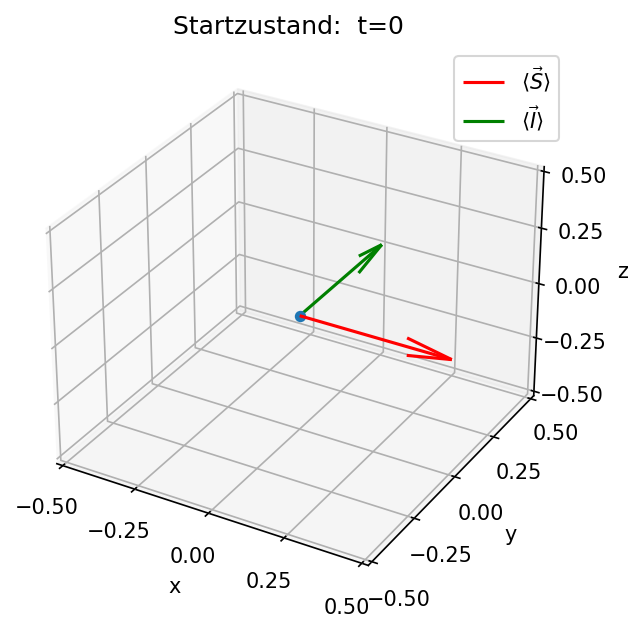
\includegraphics[width = 0.4\textwidth]{Abbildungen/Plot_Vektor_Start.png}
    \caption{gewählter Startzustand in einem 3D-Plot mit rotem Elektronenspinerwartungswert und grünem Kernspinerwartungswert als Vektoren dargestellt}
    \label{fig:Plots_Start}
\end{wrapfigure}
Es wird der Produkt-Startzustand 
\begin{align}
    \ket{\Psi_0}=\frac{1}{2}(\ket{\uparrow}_S + \ket{\downarrow}_S)(\ket{\uparrow}_I + i\ket{\downarrow}_I)
\end{align}
verwendet, welcher Äquivalent zu eine Elektronenspinerwartungswert $\langle\vec{S}\rangle$ entlang der X-Achse und orthogonal
dazu dem Kernspinerwartungswert $\langle\vec{I}\rangle$ entlang der Y-Achse, beide auf der X-Y-Ebene liegend wie in \autoref{fig:Plots_Start} zu sehen.
Unter all den möglichen Startzuständen gewählt, da dies ein sehr einfachen und anschaulichen Fall darstellt, da das Magnetfeld und beide Spinvektoren 
ein Dreibein bilden und gleich zu Beginn die Wirkung der Kopplungen unter einander durch die Orthogonalität am stärksten ist.

Dabei wird zur Lösung der Differentialgleichungen Gl. (\ref{DGL_1}) und Gl. (\ref{DGL_2}) zu lösen, wird das Runge-Kutta-Verfahren verwendet, da die 
Bewegungsgleichungen die Form besitzen:
\begin{align}
    \frac{d}{dt}\vec{f} &= \vec{f}(\vec{t}) 
\end{align}
%The parameters are chosen to approximately reflect the experimental
%setup given by Greilich et al. [33] and stay the same for the following sections unless
%stated otherwise. In previous comparisons between theory and experiment [49] T
%∗ has
%been found to be T
%∗ ≈ 1 ns
%Die Parameter werden nah am experimentellen Aufbau gegeben von Greilich et al.\cite{PMID:17901328} gewählt, d.h. wir nehmen an,
In vorherigen Vergleichen zwischen Experiment und Theorie ergab sich für die charakteristische Zeit $T^*\approx 1 \thinspace$ns\cite{PhysRevB.89.045317}, 
woraus für die Heisenbergkopplungskonstante $A = \sqrt{\frac{4}{3}}\cdot 10^9 \frac{1}{s}$ folgt. Die Zeeman-Konstante beträgt hier 
$z\approx\frac{1}{800}$. Es wird ein Magnetfeld mit $B = 0.5$ T gewählt, darüber hinaus wird die Zeitspanne so lang gewählt, dass die die Umhüllende der 
summierten Spinlänge $|\langle \left( \vec{S}+\vec{I} \right)\rangle |$  der exakten Lösung in \autoref{fig:Plots_Spinlength} ihr erstes Minimum 
überschreitet.
\begin{figure}[h]
    \centering
    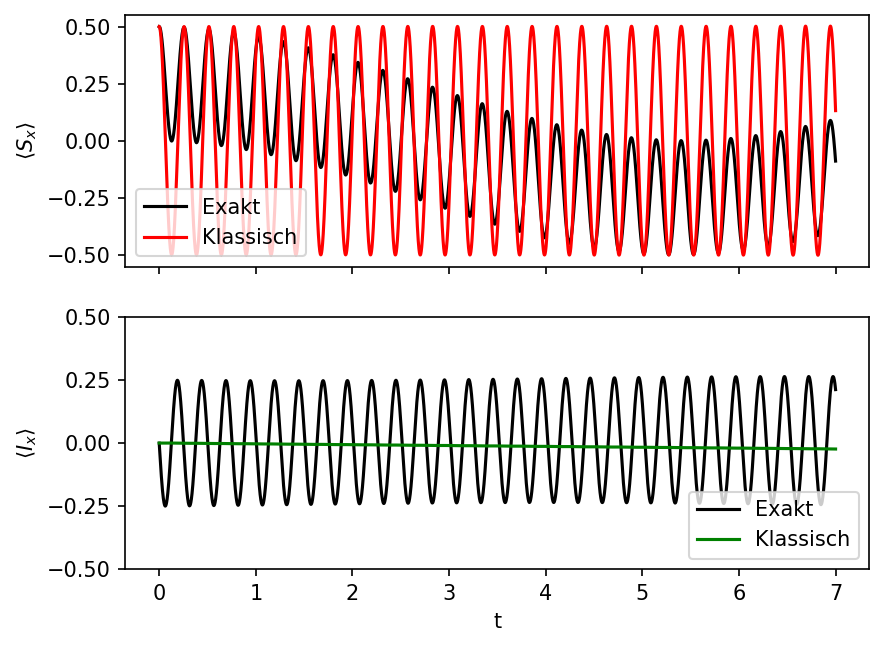
\includegraphics[width = 0.45\textwidth]{Abbildungen/Plot_Sx.png}
    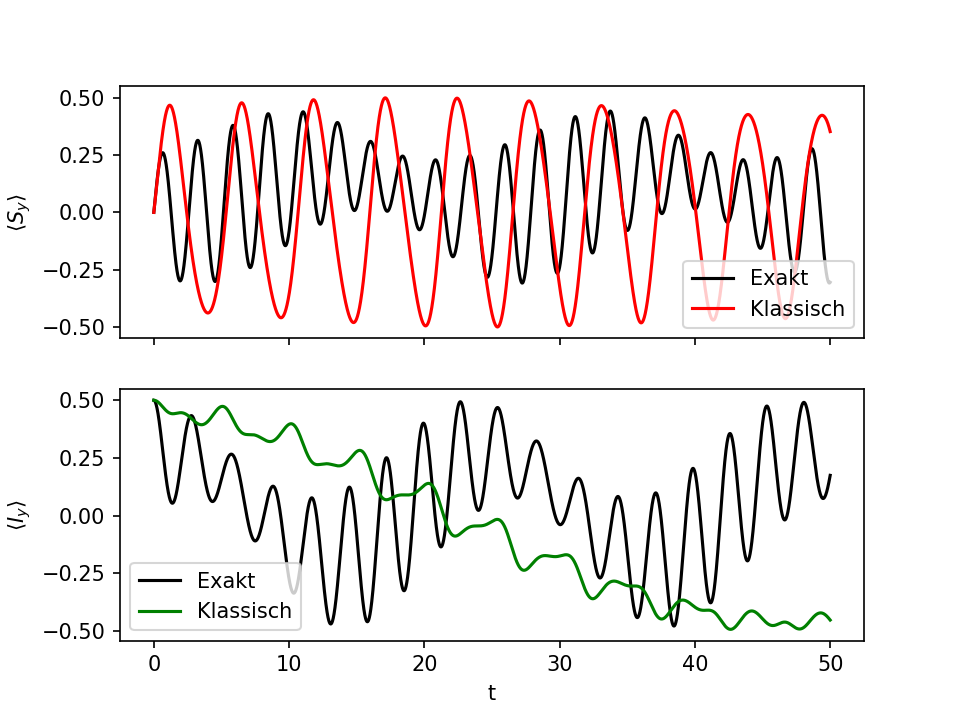
\includegraphics[width = 0.45\textwidth]{Abbildungen/Plot_Sy.png}
    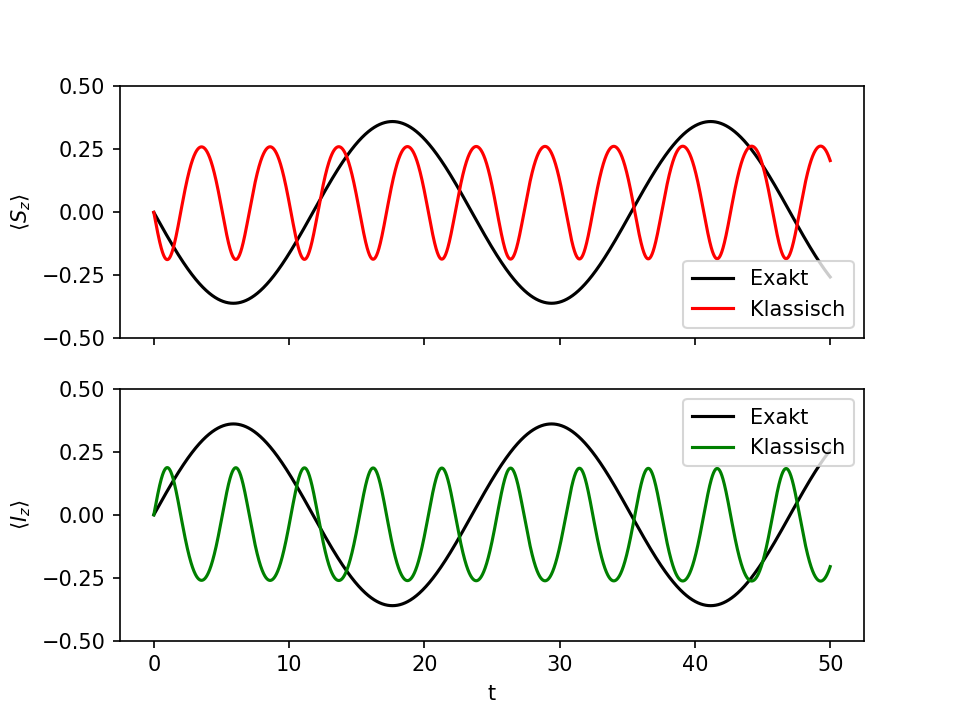
\includegraphics[width = 0.45\textwidth]{Abbildungen/Plot_Sz.png}
    \caption{Spin-Erwartungswerte des Elektronenspins S (Rot) und des Kernspins (Grün) und der jeweils exakten quantenmechanischen Lösung
    (Schwarz) gegen die Zeit t aufgetragen für die Parameter: $B = 0.5$ T, $T^*= 1 \thinspace$ns, $A_k = \sqrt{\frac{4}{3}}\cdot 10^9 \frac{1}{s}$,
    $z=\frac{1}{800}$}
    \label{fig:Plots_2D}
\end{figure}

Aus \autoref{fig:Plots_2D} im unteren Panel ist sehr gut zu erkennen, dass durch die Heisenbergkopplung die Spinerwartungswerte $\langle\hat{S}_z \rangle$ 
und $\langle\hat{I}_z \rangle$ um den Nullpunkt oszillieren und sehr kleine Amplituden besitzen, worauf geschloßen werden kann, dass die 
Spins einigermaßen auf der X-Y-Ebene verweilen und die Frequenz der klassischen Lösung deutlich größer ist als bei der Exakten.
\begin{figure}[h!]
    \centering
    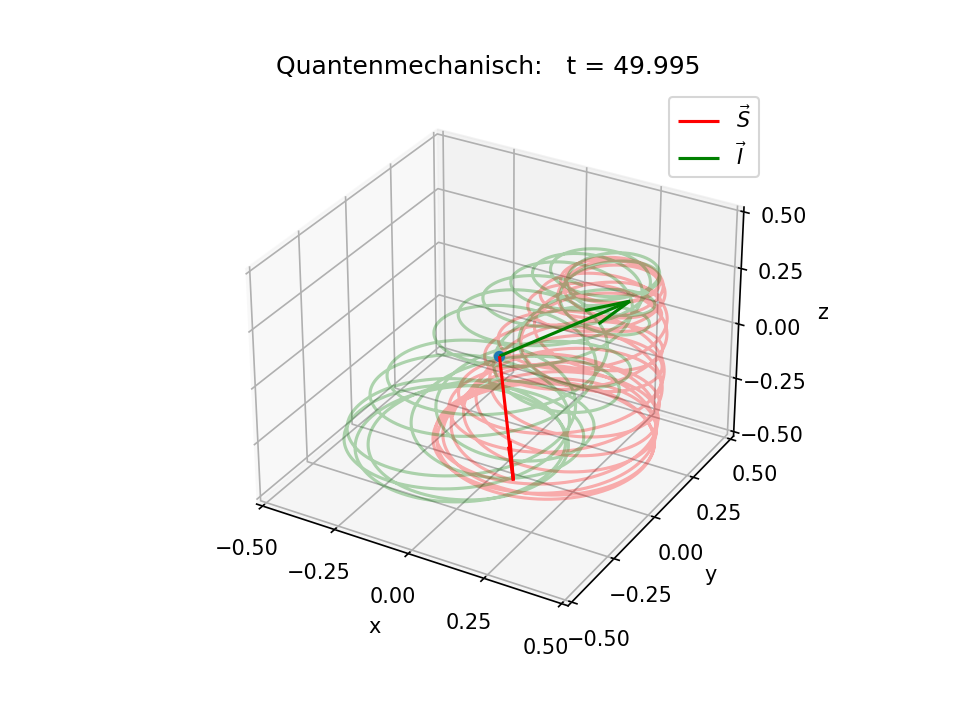
\includegraphics[width = 0.45\textwidth]{Abbildungen/Plot_Vektor_Quant.png}
    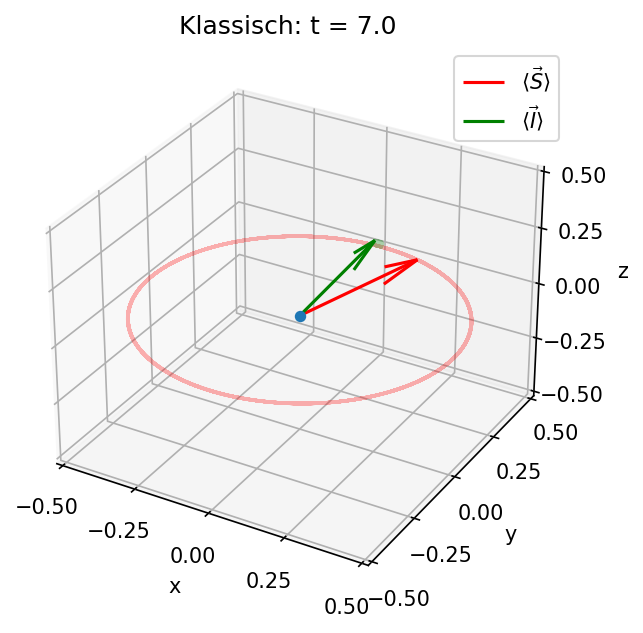
\includegraphics[width = 0.45\textwidth]{Abbildungen/Plot_Vektor_Klassisch.png}
    \caption{Spinerwartungswerte als Vektoren zum Endzeitpunkt des betrachten Zeitraums zum genannten Startzustand samt abgefahrener Spur der
    quantenmechanischen Lösung (Links) und der klassischen Lösung (Rechts) für die Parameter: $B = 0.5$ T, $T^*= 1 \thinspace$ns, $A_k = \sqrt{\frac{4}{3}}\cdot 10^9 \frac{1}{s}$,
    $z=\frac{1}{800}$}
    \label{fig:Plots_3D}
\end{figure}
% Kreisbahnen als Verschränkung. Kreiszentren präzedieren. Kreiszentrumposition aus logischen gründen anhand der addierten Spinlänge erkennbar.

Wie für die klassische Lösung zu erwarten, präzedieren Elektronen- und Kernspin um das in z-Achse ausgerichtete Magnetfeld, wobei durch die stärkere Kopplung
die Larmorfrequenz für das Elektron deutlich größer ist. Dies macht sich besonders deutlich in \autoref{fig:Plots_2D} in den oberen beiden 
Panels, wo die grüne Kurve (Kernspin) einer Geraden gleicht und zeitglich im selben Zeitintervall die rote Kurve (Elektron) mehrere Oszilattionen vollführt; 
oder wie in \autoref{fig:Plots_3D}, wo der grüne Spurverlauf (Kernspin) marginal kurz ist im Vergleich zur roten Kreisspur (Elektron), 
wo der Elektronenspin schon mindestens eine Kreisbahn abgefahren ist.\\ 
\begin{figure}[h]
    \centering
    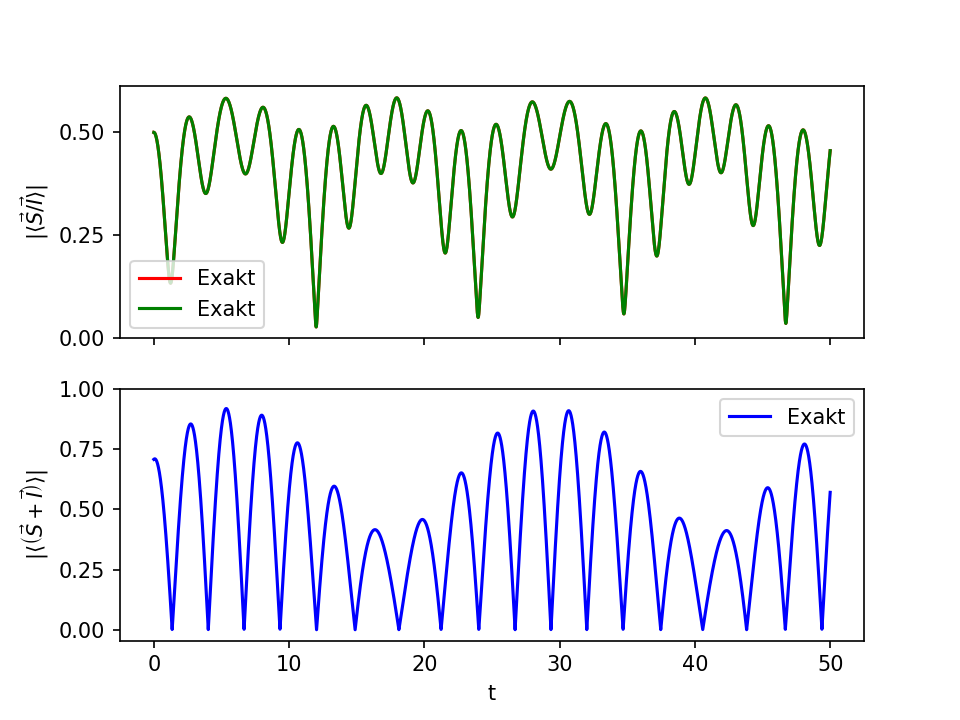
\includegraphics[width = 0.45\textwidth]{Abbildungen/Plot_Spin_length.png}
    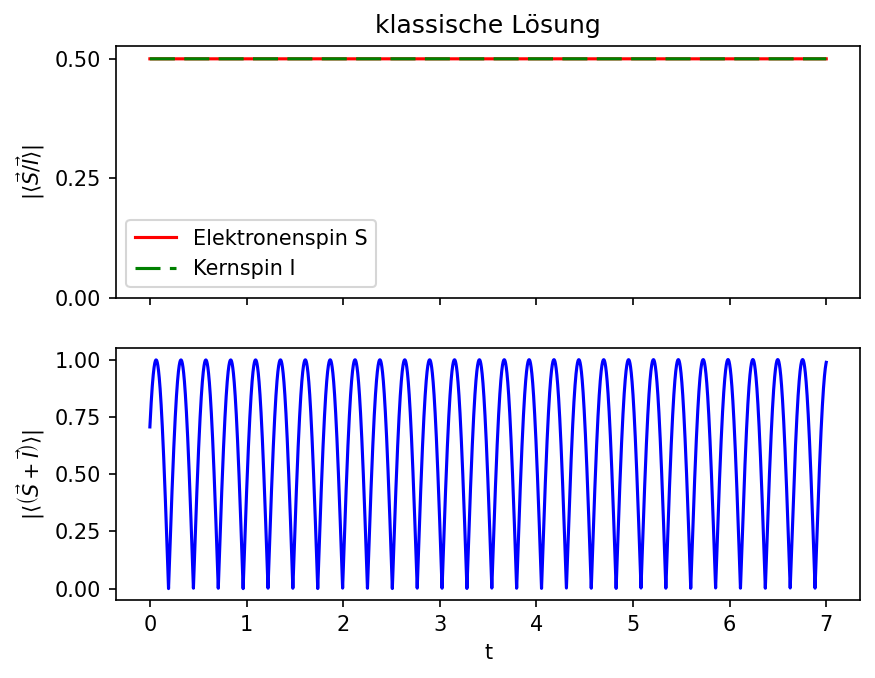
\includegraphics[width = 0.45\textwidth]{Abbildungen/Plot_Spin_length_Klassisch.png}
    \caption{Spinlängen-Erwartungswert der Einzelspins und addierten Spins des Kern-und Elektronenspins der exakten Lösung(links) und der klassischen 
    Lösung(rechts) gegen die Zeit aufgetragen für die Parameter: $B = 0.5$ T, $T^*= 1 \thinspace$ns, $A_k = \sqrt{\frac{4}{3}}\cdot 10^9 \frac{1}{s}$,
    $z=\frac{1}{800}$}
    \label{fig:Plots_Spinlength}
\end{figure}

Die exakte Lösung berücksichtigt die Verschränkung beider Spins, welches sich hauptaugenscheinlich durch Veränderungen der Einzelspinlängen ausdrückt 
wie in \autoref{fig:Plots_Spinlength} zu sehen. Dabei sind beide Spinlängen zu jedem Zeitpunkt identisch, was am totalen 
Überlappen beider Plots zu sehen ist; dasselbe gilt auch für den klassischen Fall, wobei die Spinlängen konstant bei 0.5 bleiben.\\
In \autoref{fig:Plots_3D} ist sehr gut zu erkennen, dass anders als im klassischen Fall die Spins Kreisbahnen abfahren, dessen Mittelpunkte nicht 
im Ursprung liegen, sondern gerade mittig zwischen Ursprung und maximaler Spinlänge. Trotzdessen ist eine Larmor-Präzessionsbewegung wie im Klassischen 
zu beobachten, in der nicht die Spinerwartungswerte präzedieren, sondern die jeweiligen Kreismittelpunkte, was zu den charakteristschen Schlaufen führt.\\
Dabei präzediert der Elektronenspin wie zu erwarten um einiges schneller als der schwachgekoppelte Kernspin um das Magnetfeld. Damit lässt sich auch 
erklären, warum die addierte Spinlänge $|\langle \left( \vec{S}+\vec{I} \right)\rangle |$ in \autoref{fig:Plots_Spinlength} eine Umhüllende mit Maximum
und Minimum besitzt. Denn genau beim Minimum liegen die Kreiszentren genau gegenüber und schließen einen Winkel von $\pi$, wodurch sie nur antiparallele
und keine parallelen Komponeneten teilen bzw. im Umkerhschluss ein Maximum beim Überlapp beider Zentren.
